% 附录章节中的特殊设置
% 公式编号
\newcounter{appequ}
\setcounter{appequ}{0}
\renewcommand\theequation{\arabic{appequ}}

% 列表设置
% \setlist[enumerate,1]{label=(\arabic*).,font=\normalsize,
\setlength{\parsep}{0ex}%段落间距
\setlength{\topsep}{1ex}%列表到上下文的垂直距离
\setlength{\itemsep}{0ex}%条目间距

\chapter{基于视觉和触觉反馈的自适应旋转运动控制器}\label{apx_1}

\appchapter{摘要}
在这项工作中,我们提出了一种自适应的控制方法实现转动操作。
这种控制方法可以通过手上操作将机器人手抓取的物体转动到期望的方向。
我们通过重力来实现旋转,让物体在一个单自由度夹持器的手指之间旋转,
并控制夹持力,以确保物体遵循参考轨迹并到达所需的角度位置。
我们使用一个视觉姿态估计系统来跟踪物体的姿态,
并且使用触觉传感器测量的力来控制抓取力。
摩擦系数误差是操纵中最常见的不确定性来源之一,
该自适应控制器根据摩擦系数的误差来修正系统参数。
实验证明,该自适应控制器在被控对象的摩擦参数存在不确定性的情况下能够成功地使被控对象旋转。

\appchapter{研究背景}
人类能够通过手指的协调运动滑动、滚动和推动物体实现在手上操纵,
即改变手上抓取的物体相对于手的位姿。
人手的协调运动可能是实现这一操作众多原因之一,
因为从机械的角度看人类的手具有高度的复杂性,
能够以相当精准的方式同时控制各个手指的运动。
在某种程度上,通过给机器人配备由多个手指和执行器组成的手,
机器人也可以实现这种内在的灵巧性。
然而,目前大多数机器人平台都只有相当简单的夹持器,
只有极少的自由度,因为它们通常鲁棒性更强、更经济、更容易控制,
而且它们还能简化运动规划和执行的复杂程度。
这样的夹持器看起来可能仅仅通过操纵手指来进行再抓取,
因此利用他们进行在手操作并不简单。

然而,这种灵巧度的不足可以使用外部灵巧来弥补。
即利用机器人的外部资源,例如外部接触、重力和惯性力,
使机器人能够执行复杂的操作任务。
外部敏捷性本质上是通过控制、交互感知和运动规划的有效结合,
使机器人能够协调夹持器硬件设计和控制的复杂性,更灵活、更主动地利用机器人的环境。

文献$^{[1-4]}$中介绍了许多说明机器人如何有效利用外部灵巧性进行在手操作的例子。
这些包括将被抓物体推到一个外部推力器上,使物体在夹持器内以可控的方式滑动。
其他的例子包括机械手加速运动,利用惯性力将物体拖到夹具内的指定位置,
以及让物体在重力作用下在机械手内滑动。

\begin{figure}[!ht]
  \centering
  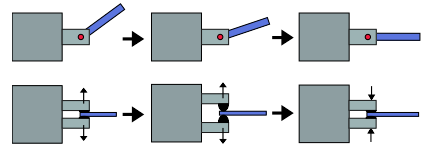
\includegraphics[scale=0.5]{appendices/pic/1-1}
  \caption*{
    \mtb{图1}通过控制两个手指的抓握所产生的夹持力来转动物体。
    上面一行展示机器人如何打开和关闭夹持器来控制由重力引起的物体旋转运动。
    该被控物体绕一个固定的旋转轴旋转,该旋转轴连接两个手指,如第二行所示。}
  \vspace{-0.3cm}
\end{figure}


在这篇论文中,我们提出了一种特殊的再抓取动作,称为旋转,
其目标是将被抓取的物体相对于机器人手旋转到一个指定角度的位置。
我们利用如图 1 所示的外部灵巧性来实现旋转,
利用被抓取物体质心产生的重力矩来旋转物体,
同时利用单自由度平行指夹具的夹持力作为制动机构来控制物体的转动轨迹。

旋转和其他在手操作的主要难题之一是如何处理未知的摩擦参数。
这是一种常见的情况,因为机器人可能需要抓取新对象或工具。
此外,由于摩擦参数与接触几何形状和压力分布等因素有关,
因此在实际测量时可能会有困难。

这激发了我们工作的主要动力。我们使用一个闭环自适应控制器进行旋转,
该控制器处理扭转摩擦参数估计不准确的问题。该控制方案需要用到视觉跟踪和
指尖触觉传感器。相较与我们之前使用闭环控制的方法$^{[5]}$,我们这次不再依耐一
些假设,如输入量的饱和。而且我们作出了以下改进,实现了增强的跟踪控制性能:

\begin{itemize}
  \item 利用软指力学改进了扭转摩擦模型。
  \item 结合触觉传感器来控制夹持力。
  \item 扭 转 摩 擦 系 数 的 实 时 修 正 。
				这 使 我 们 能 够 在 给 定 的 初 始 估 计 值 有误差的情况下,
				成功地旋转物体。
\end{itemize}


本文主要内容如下:第二节介绍该问题的相关研究工作,
第三节介绍系统的接触和动力学模型,第四节给出自适应控制律,第五节给出实验结果。
最后,我们在第六部分提出了我们的结论和未来的工作计划。

